\chapter{عمل تطبيقي : الإظهار الطيفي للصوت}

هذا العمل التطبيقي سيقترح عليك التعامل مع الـ\textenglish{SDL}
و الـ\textenglish{FMOD}
في نفس الوقت. هذه المرّة، لن نعمل على لعبة. كما نعرف فالـ\textenglish{SDL}
مخصصة لهذا، لكن يمكن استعمالها في ميادين أخرى. سيقوم هذا الفصل بإثبات أنها صالحة لأجل أشياء أخرى.

سنحقق هنا إظهاراً للطيف الصوتي بالـ\textenglish{SDL}.
يتوقّف هذا على إظهار تركيبة الصوت الذي نشغّله، مثلاً موسيقى. نجد هذه الخاصية في كثير من برامج قراءة الأصوات. إنه أمرٌ ممتع و ليس بقدر الصعوبة التي يبدو عليها !

سيسمح لك هذا الفصل بالعمل على مفاهيم قُمنا باستكشافها مؤخّراً :

\begin{itemize}
	\item التحكّم في الوقت.
	\item المكتبة 
	\textenglish{FMOD}.
\end{itemize}

سنتعرّف علاوة على ذلك، على كيفية التعديل على مساحة بيكسلا ببيكسل.

الصورة التالية تعطيك مظهراً للبرنامج الذي سنكتبه في هذا الفصل.

\begin{figure}[H]
	\centering
	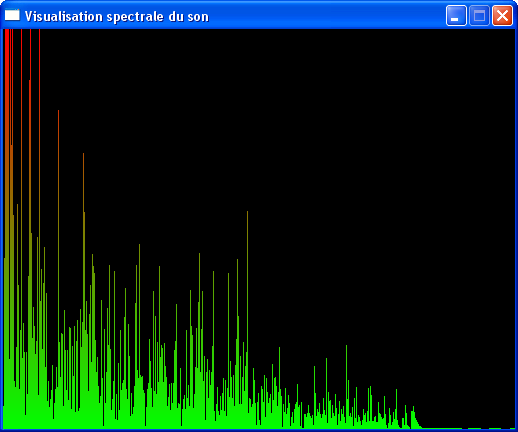
\includegraphics[width=0.8\textwidth]{Chapter_III-9_Window-spectral}
\end{figure}

هو نوع الإظهار الذي نجده في قارئي الأصوات كـ\textenglish{Winamp}،
\textenglish{Windows Media Player} أو \textenglish{AmaroK}.\\
كما قلتُ لك إن الأمر ليس صعبَ التحقيق. على عكس العمل التطبيقي الخاص بـ\textenglish{Mario Sokoban}،
هذه المرّة ستقوم بنفسك بالعمل. سيمثّل هذا بالنسبة إليك تمريناً جيداً.

\section{التعليمات}

التعليمات بسيطة. إتّبعها خطوة بخطوة بالترتيب، و لن تواجه أي مشاكل.

\subsection{قراءة ملف \textenglish{MP3}}

لكي تبدأ، يجب عليك إنشاء برنامج يقوم بقراءة ملف
\textenglish{MP3}. ليس عليك سوى إعادة
الأغنية 
"\textenglish{Home}"
للمجموعة
"\textenglish{Hype}"
و التي استعملناها في الفصل الخاص بـ\textenglish{FMOD}
لتلخيص كيفية عمل تشغيل الموسيقى.

إذا اتّبعت جيّدا الفصل حول
\textenglish{FMOD}،
لا تحتاج أكثر من بضعة دقائق لكي تقوم بالعملية. أنصحك بالمناسبة أن تقوم بنقل الملف
\textenglish{MP3}
إلى مجلّد المشروع.

\subsection{استرجاع المعلومات الطيفية للصوت}

لكي نعرف كيف يعمل الإظهار الطيفي للصوت، من الواجب أن أشرح لك كيفية يعمل الأمر من الداخل (بشكل تقريبي فقط، و إلا سندخل في درس رياضيات).

يمكن أن يتم تقسيم الصوت إلى ترددات 
(\textenglish{Frequencies}).
بعض الترددات منخفضة، بعضها متوسطة و بعضها مرتفعة. ما سنقوم به في عملية الإظهار هو إظهار كمية كلّ واحدة من الترددات على شكل شرائط و كلّما يكون الشريط كبيراً، كلما يكون التردد مستعملاً أكثر :

\begin{figure}[H]
	\centering
	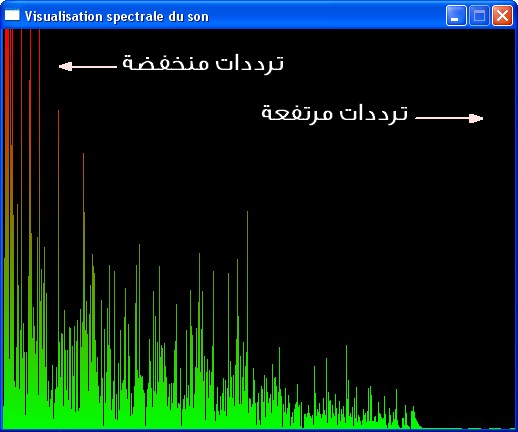
\includegraphics[width=0.8\textwidth]{Chapter_III-9_Frequencies}
\end{figure}

على يسار النافذة، نقوم بإظهار الترددات المنخفضة، و على اليمين الترددات المرتفعة.

\begin{question}
لكن كيف نسترجع كميّة كلّ تردد ؟
\end{question}

ستهتم
\textenglish{FMOD}
بهذا العمل. يمكننا استدعاء الدالة
\InlineCode{FMOD\_Channel\_GetSpectrum}
ذات النموذج :

\begin{Csource}
FMOD_RESULT FMOD_Channel_GetSpectrum(
	FMOD_CHANNEL *  channel,
	float *  spectrumarray,
	int  numvalues,
	int  channeloffset,
	FMOD_DSP_FFT_WINDOW  windowtype
);
\end{Csource}

و هاهي المعاملات التي تحتاجها الدالة :

\begin{itemize}
	\item القناة التي تشتغل فيها الموسيقى. يجب إذا استرجاع مؤشّر نحو هذه القناة.
	\item جدول
	\InlineCode{float}.
	يجب أن يتم حجز الذاكرة من أجل هذا الجدول مسبّقاً، بشكل ثابت أو حيّ، لكي نسمح لـ\textenglish{FMOD}
	بملئه بشكل صحيح.
	\item حجم الجدول. يجب أن يكون حجم الجدول إجبارياً عبارة عن قوّة للعدد 2، مثلا 512.
	\item يسمح هذا المعامل بتعريف بأي مخرج نحن مهتمون. مثلاً لو أننا في
	\textenglish{stereo}،
	فـ$ 0 $ تعني اليسار و $ 1 $ تعني اليمين.
	\item هذا المعامل معقّد قليلاً، و لا يهمّنا حقيقة في هذا الفصل. سنكتفي بإعطائه القيمة\\ 
	\InlineCode{FMOD\_DSP\_FFT\_WINDOW\_RECT}.
\end{itemize}

\begin{information}
تذكير : النوع
\InlineCode{float}
هو نوع عشري، مثل
\InlineCode{double}.
الاختلاف بين الاثنين يكمن في كون الـ\InlineCode{double}
أكثر دقّة من الآخر، لكن في حالتنا يكفينا الـ\InlineCode{float}.
هذا الأخير مستعمل من طرف
\textenglish{FMOD}
هنا. و لذلك، هو ما سنستعمله نحن أيضاً.
\end{information}

بشكل واضح، نعرّف جدول الـ\InlineCode{float} :

\begin{Csource}
float spectrum[512];
\end{Csource}

ثم، حين يتم تشغيل الموسيقى، نطلب من 
\textenglish{FMOD}
ملء جدول الأطياف بالقيام مثلاً بـ :

\begin{Csource}
FMOD_Channel_GetSpectrum(channel, spectrum, 512, 0, FMOD_DSP_FFT_WINDOW_RECT);
\end{Csource}

يمكننا بعد ذلك تصفّح الجدول لكي نتحصّل على قيم الأطياف :

\begin{Csource}
spectrum[0] // The lowest frequency (Left)
spectrum[1]
spectrum[2]
...
spectrum[509]
spectrum[510]
spectrum[511] // The highest frequency (Right)
\end{Csource}

كلّ تردد هو عبارة عن عدد عشري محصور بين $ 0 $ (لا شيء) و $ 1 $ (قيمة قصوى). ينصّ عملك على إظهار كلّ شريط سواء كان قصيراً أو كبيراً بدلالة القيمة التي تحتويها كلّ من خانات الجدول.

مثلاً، إذا كانت القيمة هي $ 0.5 $ يجدر بك رسم شريط يكون علّوه مساوياً لنصف علوّ النافذة. إذا كانت القيمة هي $ 1 $، فسيأخذ الشريط كلّ علو النافذة.

بشكل عام، تكون القيم ضعيفة (أكثر قرباً من $ 0 $ على $ 1 $). أنصحك بضرب كلّ القيم بـ20 لكي ترى الطيف بشكل أفضل.\\
احذر : إذا قمت بهذا، تأكد بأنك لن تتجاوز $ 1 $ (قم بتدوير القيمة إلى $ 1 $ إذا احجت إلى ذلك). إذا وجدت أنك تتعامل مع أعداد تفوق $ 1 $، فقد تواجه مشاكل لاحقاً في رسم الشرائط العموديّة لاحقا !

\begin{question}
لكن يجدر بالشرائط أن تتحرّك في نفس الوقت الذي يتم فيه تشغيل الصوت، أليس كذلك ؟ بما أن الصوت يتحرّك كلّ الوقت، يجب تحديث الصورة الرسومية، ما العمل ؟
\end{question}

سؤال جيد. في الواقع، الجدول الخاص المتكون من 
512 \InlineCode{float}
الذي ترجعه لنا
\textenglish{FMOD}
يتغيّر كل 25 مث (لكي نكون في نفس الفاصل الزمني بالنسبة للصوت الحالي). يجب إذا في الشفرة المصدرية أن تعيد قراءة جدول الـ512
\InlineCode{float}
 (بإعادة استدعاء
\InlineCode{FMOD\_Channel\_GetSpectrum}
 كلّ 25 مث)، ثم تقوم بتحديث رسمك ذي الشرائط.
 
أعد قراءة الفصل حول التحكّم في الوقت بالـ\textenglish{SDL}
لكي تتذكّر كيفية عمل ذلك. لديك الخيار بين
\InlineCode{GetTicks}
و الـ\textenglish{callbacks}.
استعمل ما تراه أكثر سهولة لك.

\subsection{إنشاء التدرّج اللوني}

في البداية، يمكنك تحقيق الشرائط بلون موحّد. يمكنك إذا إنشاء مساحات. يجب إذا أن تكون هناك 512 مساحة : واحدة من أجل كلّ شريط. كلّ مساحة تأخذ إذا بيكسلا واحدا كعُرض. و يختلف علوّ الشرائط بدلالة شدّة كلّ تردد.

أنصحك بعدها أن تقوم بتحسين : يجب على الشريط أن يميل للأحمر كلّما زادت كثافة الصوت. أي أنه على الشريط أن يكون أخضراً من الأسفل و أحمراً من الأعلى.

\begin{question}
لكن \dots المساحة الواحدة لا يمكنها أن تأخذ سوى لونٍ واحدٍ لو عندما نستعمل الدالة
\InlineCode{SDL\_FillRect}.
لا يمكننا إنشاء تدرّح لوني !
\end{question}

في الواقع، يمكننا بالتأكيد إنشاء مساحات بعَرْض 1 بيكسل و عُلُو 1 بيكسل من أجل كلّ لون في التدرّج. لكن هذا سيأخذ بنا إلى إنشاء مساحات عديدة و لن يكون التحكّم فيها مثالياً !

كيف يمكن لنا أن نرسم بيكسلا ببيكسل ؟\\
لم أعلّمك هذا من قبل، لأنّ هذه التقنية لا تستحقّ فصلاً كاملاً. ستجد أنها في الواقع ليست صعبة. 

في الواقع، لا تقترح الـ\textenglish{SDL}
أية دالة للرسم بيكسلا ببيكسل. لكن لنا الحق في أن نكتبها بأنفسنا. لكي نقوم بهذا، يجب إتّباع هذه الخطوات النموذجية بالترتيب :

\begin{enumerate}
	\item استدع الدالة
	\InlineCode{SDL\_LockSurface}
	لنعلن للـ\textenglish{SDL}
	أننا سنقوم بالتعديل على المساحة يدوياً. هذا "يعطّل" المساحة للـ\textenglish{SDL}
	و ستكون وحدك قادراً على التحكّم فيها مادامت المساحة معطّلة.
	
	هنا، أنصحك بأن تعمل بمساحة واحدة فقط : الشاشة. إذا أردت رسم بيكسل في منطقة محددة من الشاشة، يجب عليك تعطيل المساحة 
	\InlineCode{screen} :
	
\begin{Csource}
SDL_LockSurface(screen);
\end{Csource}

	\item يمكنك بعد ذلك تغيير محتوى كلّ بيكسل من المساحة. بما أن الـ\textenglish{SDL}
	لا تقترح أية دالة للقيام بهذا، يجب أن نكتبها بأنفسنا في البرنامج.
	
	سأعطيك هذه الدالة، و التي استخرجتها من الملفات التوجيهية للـ\textenglish{SDL}.
	هي معقدّة أكثر لأنها تعمل على المساحة مباشرة و تتحكم في كلّ أعماق اللون الممكنة (بيتات على البيكسل). لا تحتاج لحفظها أو فهمها، قم بنسخها ببساطة في البرنامج لكي تتمكّن من استعمالها :
	
\begin{Csource}
void setPixel(SDL_Surface *surface, int x, int y, Uint32 pixel)
{
	int bpp = surface->format->BytesPerPixel;
	
	Uint8 *p = (Uint8 *)surface->pixels + y * surface->pitch + x * bpp;
	
	switch(bpp) {
		case 1:
		*p = pixel;
		break;
		
		case 2:
		*(Uint16 *)p = pixel;
		break;
		
		case 3:
		if(SDL_BYTEORDER == SDL_BIG_ENDIAN) {
			p[0] = (pixel >> 16) & 0xff;
			p[1] = (pixel >> 8) & 0xff;
			p[2] = pixel & 0xff;
		} else {
			p[0] = pixel & 0xff;
			p[1] = (pixel >> 8) & 0xff;
			p[2] = (pixel >> 16) & 0xff;
		}
		break;
		
		case 4:
		*(Uint32 *)p = pixel;
		break;
	}
}
\end{Csource}
\end{enumerate}

هي سهلة الاستعمال. ابعث لها المعاملات التالية :

\begin{itemize}
	\item المؤشّر نحو المساحة التي تريد التعديل عليها (يجب أن تكون معطّلة بواسطة
	\InlineCode{SDL\_LockSurface}).
	\item وضعية الفاصلة الخاصة بالبيكسل الذي نريد التعديل عليه في المساحة
	(\InlineCode{x}).
	\item وضعية الترتيبة الخاصة بالبيكسل الذي نريد التعديل عليه في المساحة
	(\InlineCode{y}).
	\item اللون الجديد الذي نعطيه للبيكسل. يجب أن يكون هذا اللون بصيغة
	\InlineCode{Uint32}.
	يمكنك إذا توليده بالاستعانة بالدالة
	\InlineCode{SDL\_MapRGB}
	التي تتقننها جيداً الآن.
	\item أخيراً، حينما تنتهي من العمل على المساحة، يجب ألا تنسى أن تزيل تعطيلها باستدعاء\\ 
	\InlineCode{SDL\_UnlockSurface}.
\end{itemize}

\begin{Csource}
SDL_UnlockSurface(screen);
\end{Csource}

\subsection{شفرة  ملخّصة للمثال}

لو نلخّص، ستجد بأن كلّ شيء سهل.\\
هذه الشفرة ترسم بيكسلا أحمرا في منتصف المساحة
\InlineCode{screen}
(أي في منتصف النافذة).

\begin{Csource}
SDL_LockSurface(screen); // We lock the surface
setPixel(screen, screen->w / 2, screen->h / 2, SDL_MapRGB(screen->format, 255, 0, 0)); // We draw a red pixel in the middle of the screen
SDL_UnlockSurface(screen); // We unlock the surface
\end{Csource}

من هذه القاعدة، يجدر بك أن تتمكن من تحقيق التدرّج اللوني من الأخضر للأحمر (يجب أن تستعمل الحلقات التكرارية).

\section{التصحيح}

إذا، كيف وجدت الموضوع ؟ ليس صعب الفهم، يجب فقط القيام ببعض الحسابات، خاصة من أجل تحقيق التدرّج اللوني. مستوى التمرين هو مستوً عام، يجب فقط أن تفكّر أكثر. 

بعض الأشخاص يأخذون وقتاً أطول من آخرين لإيجاد التصحيح. إذا لم تتمكّن من حلّ التمرين، هذا ليس سيئاً. ما يهمّ هو أن ننتهي بالوصول إلى هدفنا. مهما كان المشروع الذي تعمل عليه، فسيكون هناك بالتأكيد أوقات نجد فيها أنه لا ينقصنا أن نجيد البرمجة لكي نتمكّن من حلّ المشكل، يجب أيضاً أن نكون منطقيين و نجيد التفكير.

سأعطيك الشفرة المصدرية الكاملة. لقد علّقت عليها بشكل كافٍ :

\begin{Csource}
#include <stdlib.h>
#include <stdio.h>
#include <SDL/SDL.h>
#include <fmodex/fmod.h>
#define WINDOW_WIDTH 512 // MUST stay equal to 512 because there are 512 bars corresponding to 512 floats
#define WINDOW_HIGHT 400 // You can change this.
#define RATIO (WINDOW_HIGHT / 255.0)
#define LIMIT_TIME_TO_REFRESH 25 // Time in ms between two updates of the graph (25 is the minimum)
#define SPECTERUM_SIZE 512
void setPixel(SDL_Surface *surface, int x, int y, Uint32 pixel);
int main(int argc, char *argv[])
{
	SDL_Surface *screen = NULL;
	SDL_Event event;
	int cont = 1, barHeight = 0, currentTime = 0, previousTime = 0, i = 0, j = 0;
	float spectrum[SPECTERUM_SIZE];
	/* Initializing FMOD:
	Load FMOD, the music and start playing the music
	*/
	
	FMOD_SYSTEM *system;
	FMOD_SOUND *music;
	FMOD_CHANNEL *channel;
	FMOD_RESULT result;
	FMOD_System_Create(&system);
	FMOD_System_Init(system, 1, FMOD_INIT_NORMAL, NULL);
	// We open the music
	result = FMOD_System_CreateSound(system, "hype_home.mp3", FMOD_SOFTWARE | FMOD_2D | FMOD_CREATESTREAM, 0, &music);
	// We check if it has been opened correctly (IMPORTANT)
	if (result != FMOD_OK)
	{
		fprintf(stderr, "Can't read the mp3 file\n");
		exit(EXIT_FAILURE);
	}
	// We play the music
	FMOD_System_PlaySound(system, FMOD_CHANNEL_FREE, music, 0, NULL);
	
	// We get the channel pointer
	FMOD_System_GetChannel(system, 0, &channel);
	/*
	Initializing the SDL:
	---------------------
	We load the SDL, open a window and write in its title bar.
	We get also a pointer to the surface screen which will be the only surface to use in this program 
	*/
	SDL_Init(SDL_INIT_VIDEO);
	screen = SDL_SetVideoMode(WINDOW_WIDTH, WINDOW_HIGHT, 32, SDL_SWSURFACE | SDL_DOUBLEBUF);
	SDL_WM_SetCaption("Visualisation spectrale du son", NULL);
	// Main loop	
	while (cont)
	{
		SDL_PollEvent(&event); // We have to use PollEvent because we don't have to wait for the user's event to refresh the window
		switch(event.type)
		{
			case SDL_QUIT:
			cont = 0;
			break;
		}
		// We clear the screen every time before drawing the graph (black wallpaper)
		SDL_FillRect(screen, NULL, SDL_MapRGB(screen->format, 0, 0, 0));
		/* Managing the time
		-----------------
		We compare between the current time and the previous one (the last iteration of the loop).
		If the difference is less than 25 ms (updating time limit)
		Then we wait until 25ms pass.
		After that, we update previousTime with the new time. */
		currentTime = SDL_GetTicks();
		if (currentTime - previousTime < LIMIT_TIME_TO_REFRESH)
		{
			SDL_Delay(LIMIT_TIME_TO_REFRESH-(currentTime-previousTime));
		}
		previousTime = SDL_GetTicks();
		/* Drawing the sound spectrum
		------------------------
		It's the most important part. We have to think a little bit before drawing the spectrum. Maybe it's hard but it's possible, here is the proof.
		We fill the 512 floats table via FMOD_Channel_GetSpectrum()
		Then we work pixel by pixel on the surface screen to draw the bars.
		We make a first loop to browse the window in width.
		The second loop browses the window in height to draw the bars.
		*/
		
		/* We fill the 512 floats table. I've chosen to be interested in the left output */
		FMOD_Channel_GetSpectrum(channel, spectrum, SPECTERUM_SIZE, 0, FMOD_DSP_FFT_WINDOW_RECT);
		SDL_LockSurface(screen);
		/* We block the surface screen because we're going to directly modify its pixels */
		
		/* LOOP 1 : We browse the window in width (for every vertical bar) */
		for (i = 0 ; i < WINDOW_WIDTH ; i++)
		{
			/* We calculate the vertical bar's height that we're going to draw.
			spectrum[i] will return a number between 0 and 1 that we're going to multiply by 20 to zoom in order to have a better view (As I said).
			
			The, we multiply by WINDOW_HEIGHT so the bar will be expanded comparing to the window's size. */
			
			barHeight = spectrum[i] * 20 * WINDOW_HIGHT;
			/* We verify that the bar doesn't exceed the height of the window
			If it's the case, we crop the bar so it become equal to the window's height. */
			if (barHeight > WINDOW_HIGHT)	
				barHeight = WINDOW_HIGHT;
			/* LOOP 2 : we browse in height the vertical bar to draw it */
			
			for (j = WINDOW_HIGHT - barHeight ; j < WINDOW_HIGHT ; j++)	
			{
				/* We draw each pixel of the bar with the right colour.
				We simply vary the red and green colours, each one in a different way.
				
				j doesn't vary between 0 and 255 but between 0 and WINDOW_HEIGHT.
				
				If we want to adapt it proportionally to the window's height, we can simply calculate j / RATIO, where RATIO is equal to (WINDOW_HEIGHT / 255.0).
				
				It tooks for me 2-3 minutes so I can find the write calculation to do, every one can do it. You just have to think a little bit */
				
				setPixel(screen, i, j, SDL_MapRGB(screen->format, 255 - (j / RATIO), j / RATIO, 0));
			}
		}
		SDL_UnlockSurface(screen); /* We have finished working on the screen, we block the surface */
		SDL_Flip(screen);
	}
	/* The program is finished.
	We free the music from the memory
	And we close FMOD and SDL */
	
	FMOD_Sound_Release(music);
	FMOD_System_Close(system);
	FMOD_System_Release(system);
	SDL_Quit();
	return EXIT_SUCCESS;
}
/* The function setPixel lets us draw a surface pixel by pixel */

void setPixel(SDL_Surface *surface, int x, int y, Uint32 pixel)
{
	int bpp = surface->format->BytesPerPixel;
	Uint8 *p = (Uint8 *)surface->pixels + y * surface->pitch + x * bpp;
	switch(bpp) 
	{
		case 1:
		*p = pixel;
		break;
		case 2:
		*(Uint16 *)p = pixel;
		break;
		case 3:
		if(SDL_BYTEORDER == SDL_BIG_ENDIAN)
		{
			p[0] = (pixel >> 16) & 0xff;
			p[1] = (pixel >> 8) & 0xff;
			p[2] = pixel & 0xff;
		} 
		else
		{
			p[0] = pixel & 0xff;
			p[1] = (pixel >> 8) & 0xff;
			p[2] = (pixel >> 16) & 0xff;
		}
		break;
		case 4:
		*(Uint32 *)p = pixel;
		break;
	}
}
\end{Csource}

يجدر بك أن تتحصّل على نتيجة تشبه الصورة التالية :

\begin{figure}[H]
	\centering
	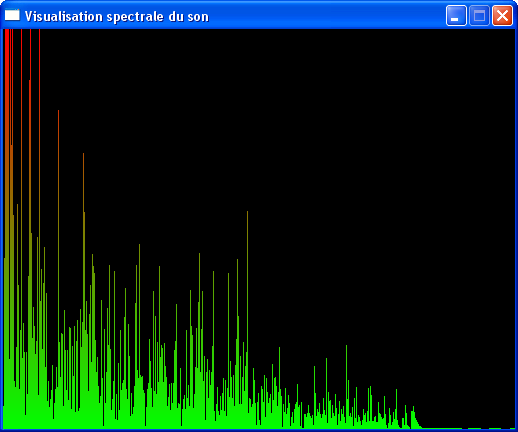
\includegraphics[width=0.8\textwidth]{Chapter_III-9_Window-spectral}
\end{figure}

من المعلوم أن النتيجة المرئية أفضل لتقدير النتيجة. أنصحك بالاطلاع عليها من هنا :

\textenglish{\url{https://openclassrooms.com/uploads/fr/ftp/mateo21/spectre.html} (4.3 Mo)}

لاحظ أن ضغط الملف أنقص من جودة الصوت و عدد الصور في الثانية.\\
الأفضل هو أن تقوم بتحميل البرنامج كاملاً (مرفقاً بالشفرة المصدرية) لكي تجربه عندك. يمكنك حينها تقدير البرنامج في ظروف أفضل.

تنزيل الملف التنفيذي و الشفرة المصدرية الكاملة :

\url{https://openclassrooms.com/uploads/fr/ftp/mateo21/spectre.zip}

\begin{critical}
يجب قطعاً أن يكون الملف
\InlineCode{Hype\_Home.mp3}
متواجداً في مجلّد المشروع لكي يشتغل البرنامج (و إلا فسيتوقف حالاً).
\end{critical}

\section*{أفكار للتحسين}

يمكن دائما تحسين البرنامج. هنا، لدي مثلاً أفكار تمديد كثيرة يمكنها أن تصل بك إلى إنشاء برنامج صغير لقراءة الملفات
\textenglish{MP3}.

\begin{itemize}
	\item سيكون من الجيد أن نختار بأنفسنا الملف
	\textenglish{MP3}
	الذي نريد قراءته. يمكن مثلاً أن نقدّم لائحة تضم كلّ الملفات بذات الصيغة و المتواجدة في مجلّد المشروع. لم نرَ كيف نقوم بذلك، لكن يمكنك وحدك أن تكتشف ذلك. كمساعدة : استعمل المكتبة
	\textenglish{dirent}
	( قم بتضمين الملف 
	\InlineCode{dirent.h}).
	عليك بالبحث في الأنترنت لتعرف كيفيّة العمل بها.
	\item إذا كان البرنامج قادرا على التحكّم في لائحات التشغيل
	(\textenglish{Playlists})
	المشغّلة، سيكون أمراً أفضل. توجد كثير من صيغ اللائحات و أشهرها الصيغة
	\textenglish{M3U}.
	\item يمكنك إظهار اسم الـ\textenglish{MP3}
	التي أنت بصدد تشغيله في النافذة مثلاً (يجب استعمال
	\textenglish{SDL\_ttf}).
	\item يمكنك إظهار مؤشّر يشير إلى المكان في القراءة الّذي وصل إليه التشغيل، هذا ما يفعله أغلب قارئي الـ\textenglish{MP3}.
	\item يمكنك أيضاً أن تقترح التعديل على قوة الصوت.
	\item إلى آخره.
\end{itemize}

باختصار، هناك الكثير لفعله. لديك إمكانيّة إنشاء قارئي أصوات ممتازة، ليس عليك سوى كتابة الشفرة الخاصة بها !
